\documentclass[12pt, a4paper]{article}

% ── Packages ─────────────────────────────────────────────────────────
\usepackage[T1]{fontenc}
\usepackage[utf8]{inputenc}
\usepackage[english]{babel}
\usepackage{geometry}
\geometry{a4paper, margin=2.5cm, headheight=15pt}

\usepackage{amsmath, amssymb}
\usepackage{graphicx}
\usepackage{booktabs}
\usepackage{array}
\usepackage{caption}
\usepackage{subcaption}
\usepackage{float}
\usepackage{hyperref}
\usepackage{xcolor}
\usepackage{parskip}
\usepackage{titlesec}
\usepackage{fancyhdr}
\usepackage{cite}

% ── Hyperref setup ───────────────────────────────────────────────────
\hypersetup{
    colorlinks=true,
    linkcolor=blue!60!black,
    citecolor=green!50!black,
    urlcolor=blue!60!black,
}

% ── Page style ───────────────────────────────────────────────────────
\pagestyle{fancy}
\fancyhf{}
\rhead{ECE328 — Information Retrieval}
\lhead{Nikos Mavros (03741)}
\rfoot{\thepage}

% ── Section formatting ───────────────────────────────────────────────
\titleformat{\section}{\large\bfseries}{\thesection.}{0.5em}{}
\titleformat{\subsection}{\normalsize\bfseries}{\thesubsection.}{0.5em}{}

% ── Graphics path ────────────────────────────────────────────────────
\graphicspath{{../results/figures/}}

% ─────────────────────────────────────────────────────────────────────
\setlength{\emergencystretch}{3em}
\begin{document}

% ── Title page ───────────────────────────────────────────────────────
\begin{titlepage}
  \centering
  \vspace*{2cm}
  {\Large University of Thessaly \\ Department of Electrical and Computer Engineering \par}
  \vspace{1.5cm}
  {\rule{\linewidth}{0.5pt}\par}
  \vspace{0.5cm}
  {\LARGE\bfseries Information Retrieval Assignment\par}
  \vspace{0.4cm}
  {\large ECE328 — Spring 2026\par}
  \vspace{0.3cm}
  {\rule{\linewidth}{0.5pt}\par}
  \vspace{1.5cm}
  {\large\textbf{Nikos Mavros}\par}
  \vspace{0.2cm}
  {\large AEM: 03741\par}
  \vspace{0.2cm}
  {\large \href{mailto:nmavros@uth.gr}{nmavros@uth.gr}\par}
  \vfill
  {\large Submitted: June 14, 2026\par}
  \vspace{0.5cm}
  {\normalsize Submission e-mail: \href{mailto:draf@uth.gr}{draf@uth.gr}\par}
\end{titlepage}

\tableofcontents
\newpage

% ═════════════════════════════════════════════════════════════════════
\section{Part 1 — Link Analysis (4 points)}
% ═════════════════════════════════════════════════════════════════════

\subsection{Part 1A — Personalised PageRank on the 14-node graph}

\subsubsection*{Setup}

We computed Personalised PageRank on the 14-node undirected graph shown in
Figure~\ref{fig:p1a_graph}, using damping factor $a = 0.65$.
The teleportation vector $\mathbf{v}$ is non-uniform: node~14 receives
probability mass $0.5$, and the remaining $0.5$ is distributed uniformly
across the other 13 nodes ($\approx 3.85\%$ each).
All edges are bidirectional; the graph has 22 edges forming three loosely
connected clusters: a left cluster $\{1,2,3,4,5\}$, a bottom cluster
$\{6,7,8,9\}$, and a right cluster $\{10,11,12,13,14\}$, joined by
single-edge bridges.

\begin{figure}[H]
  \centering
  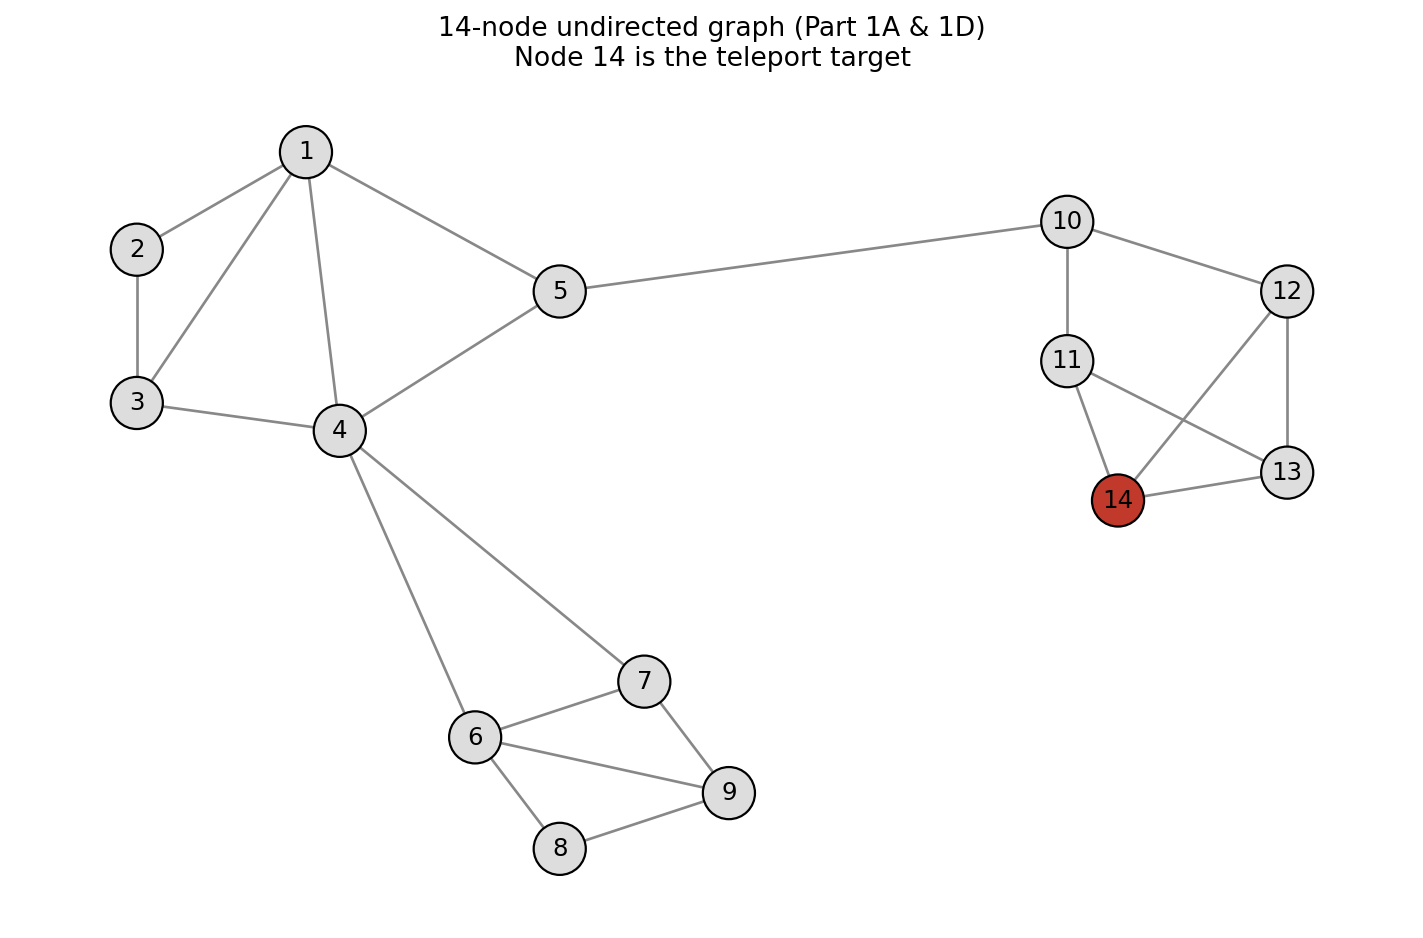
\includegraphics[width=0.72\textwidth]{p1a_graph.png}
  \caption{The 14-node undirected graph used in Parts 1A and 1D.
           Node~14 (highlighted in red) is the teleport target.}
  \label{fig:p1a_graph}
\end{figure}

\subsubsection*{Results}

\begin{figure}[H]
  \centering
  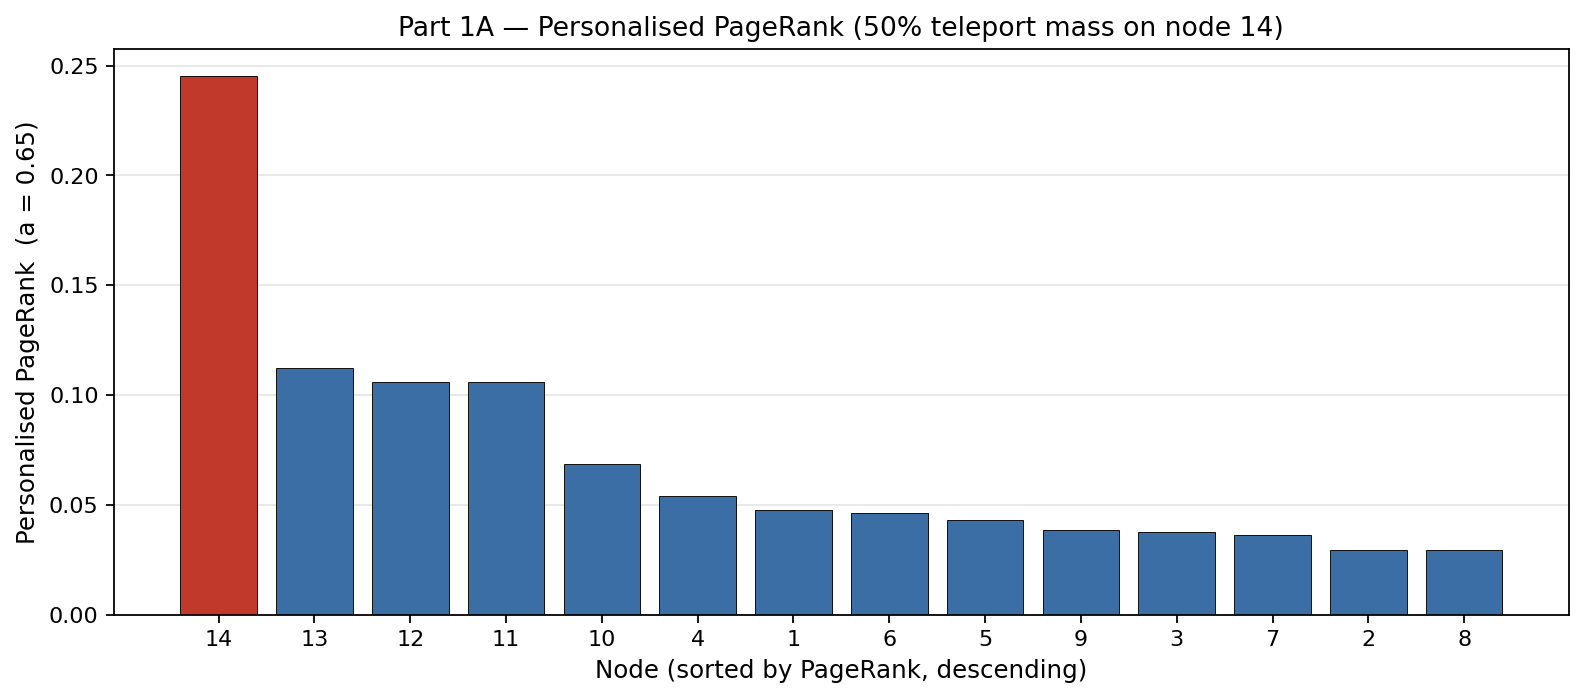
\includegraphics[width=0.95\textwidth]{p1a_pagerank_bar.png}
  \caption{Personalised PageRank scores for all 14 nodes (sorted descending).
           Node~14 is highlighted in red.}
  \label{fig:p1a_bar}
\end{figure}

The top-5 ranked nodes are reported in Table~\ref{tab:p1a}.

\begin{table}[H]
  \centering
  \caption{Top-5 Personalised PageRank scores ($a=0.65$).}
  \label{tab:p1a}
  \begin{tabular}{ccc}
    \toprule
    \textbf{Rank} & \textbf{Node} & \textbf{PageRank} \\
    \midrule
    1 & 14 & 0.2452 \\
    2 & 13 & 0.1125 \\
    3 & 12 & 0.1058 \\
    4 & 11 & 0.1058 \\
    5 & 10 & 0.0687 \\
    \bottomrule
  \end{tabular}
\end{table}

\subsubsection*{Discussion}

Node~14 ranks first by a large margin (score $0.2452$, more than double the
second-ranked node), solely due to the $50\%$ teleportation mass assigned to
it. Its immediate neighbours in the right cluster---nodes 11, 12, and 13, all
directly connected to node~14---occupy the next three positions, since random
walks that restart on node~14 immediately propagate probability mass to them.
Node~10 follows at rank~5; it acts as the gateway between the right cluster
and the rest of the graph (connected to both node~11 and node~12).

Critically, the personalisation vector overrides the topological signal:
in standard uniform-teleport PageRank, well-connected hub nodes such as
node~4 (degree~5) and node~1 (degree~4) would rank at the top; here they
fall below the entire right cluster because the repeated injections of
probability mass near node~14 flood that region.

Nodes in the bottom cluster ($\{6,7,8,9\}$) rank last, consistent with their
greater graph distance from node~14. Node~8 in particular has degree~2
(connected only to nodes 6 and 9) and no path shorter than 5 hops to
node~14, producing the lowest score overall.

% ─────────────────────────────────────────────────────────────────────
\subsection{Part 1B — Damping factor sweep on the 8-node directed graph}

\subsubsection*{Setup}

We computed PageRank on the 8-node directed graph (Figure~\ref{fig:p1b_graph})
for five damping factors $a \in \{0.55, 0.65, 0.75, 0.85, 0.95\}$.
Each configuration uses a uniform teleportation vector.
We then measured the stability of the induced rankings by computing
pairwise Kendall $\tau$ between all $\binom{5}{2} = 10$ pairs of rankings.

\begin{figure}[H]
  \centering
  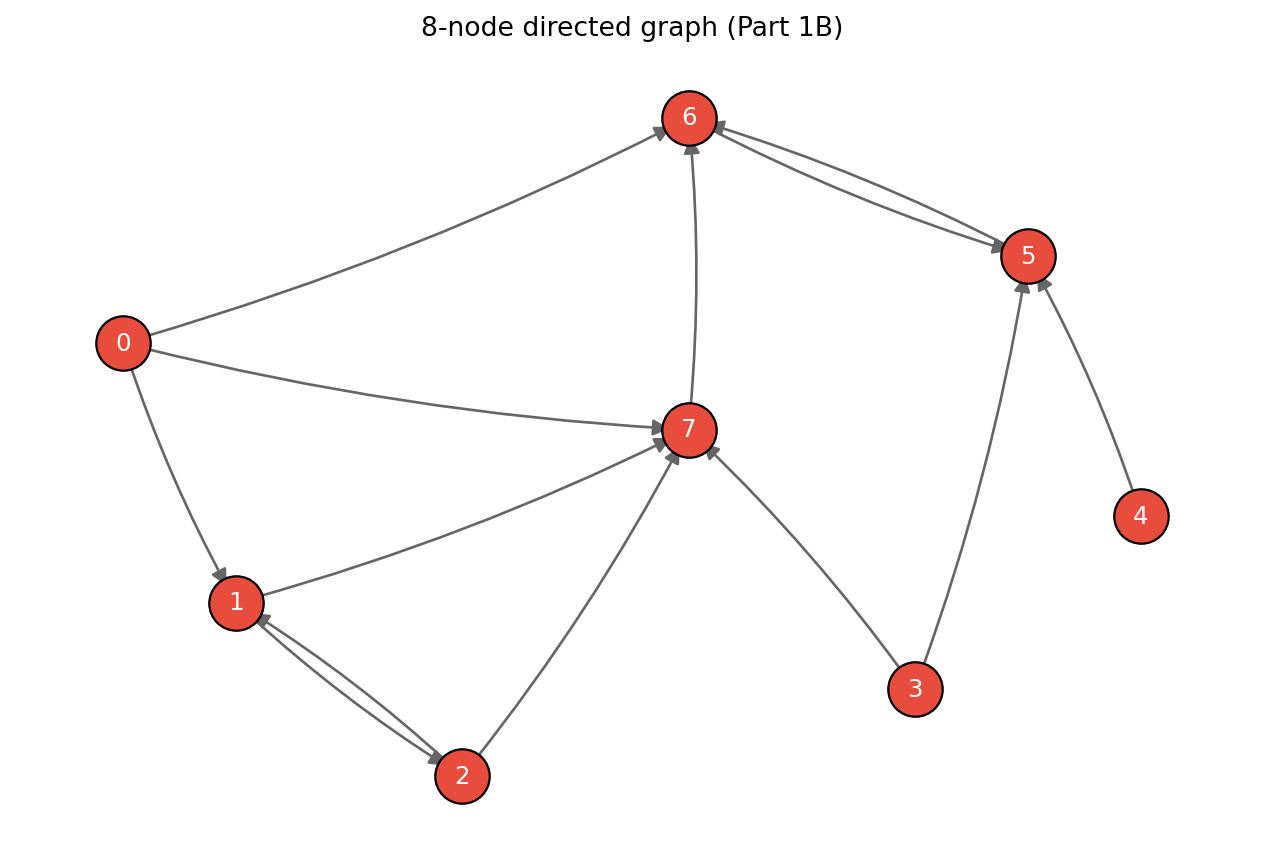
\includegraphics[width=0.60\textwidth]{p1b_graph.png}
  \caption{The 8-node directed graph used in Part~1B.}
  \label{fig:p1b_graph}
\end{figure}

\subsubsection*{Results}

Figures~\ref{fig:p1b_n0}--\ref{fig:p1b_n7} show the PageRank value of each
node as a function of the damping factor $a$, one figure per node.

\begin{figure}[H]
  \centering
  \begin{subfigure}[b]{0.48\textwidth}
    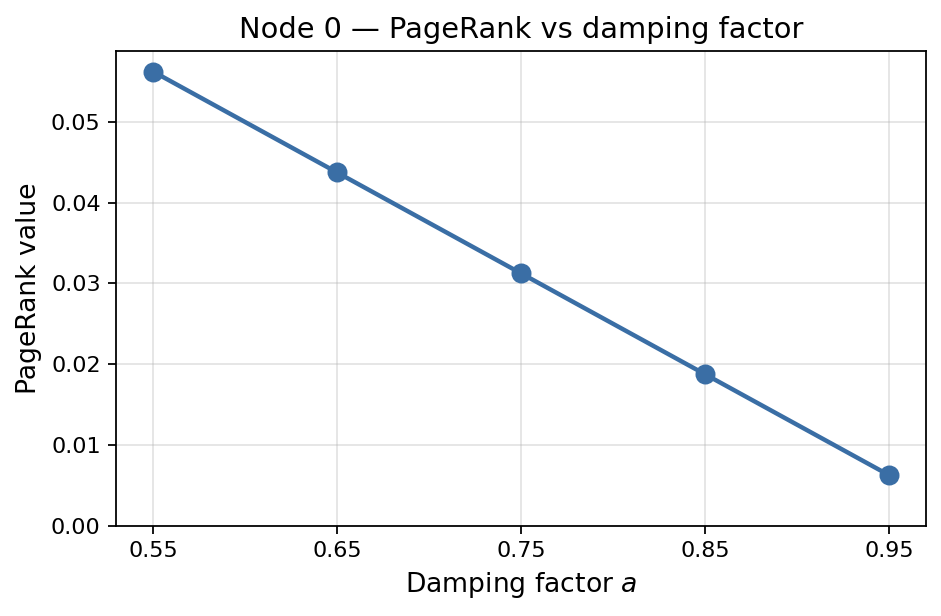
\includegraphics[width=\textwidth]{p1b_node0.png}
    \caption{Node 0}
    \label{fig:p1b_n0}
  \end{subfigure}
  \hfill
  \begin{subfigure}[b]{0.48\textwidth}
    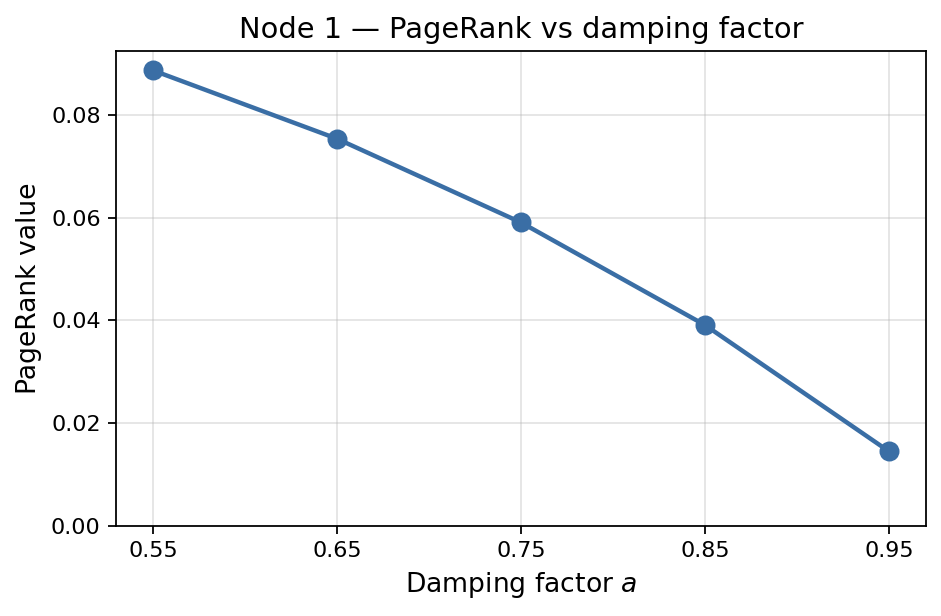
\includegraphics[width=\textwidth]{p1b_node1.png}
    \caption{Node 1}
    \label{fig:p1b_n1}
  \end{subfigure}
  \begin{subfigure}[b]{0.48\textwidth}
    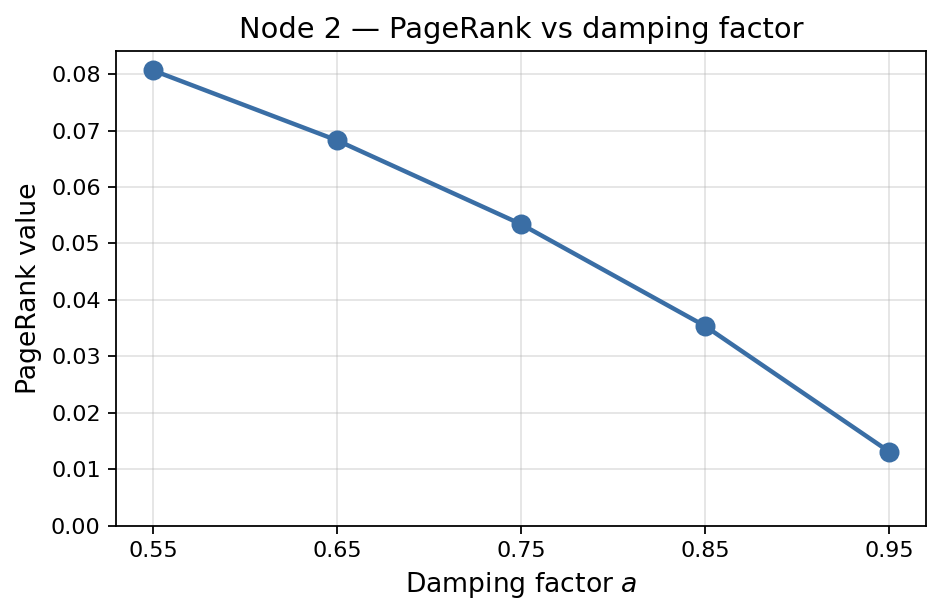
\includegraphics[width=\textwidth]{p1b_node2.png}
    \caption{Node 2}
    \label{fig:p1b_n2}
  \end{subfigure}
  \hfill
  \begin{subfigure}[b]{0.48\textwidth}
    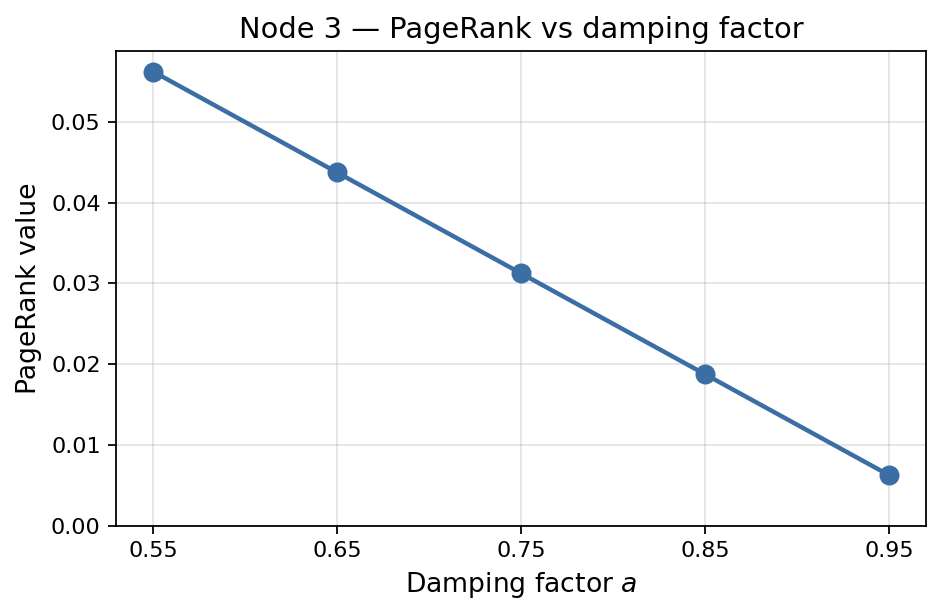
\includegraphics[width=\textwidth]{p1b_node3.png}
    \caption{Node 3}
    \label{fig:p1b_n3}
  \end{subfigure}
  \caption{Part 1B — PageRank vs damping factor, nodes 0--3.}
  \label{fig:p1b_part1}
\end{figure}

\begin{figure}[H]
  \centering
  \begin{subfigure}[b]{0.48\textwidth}
    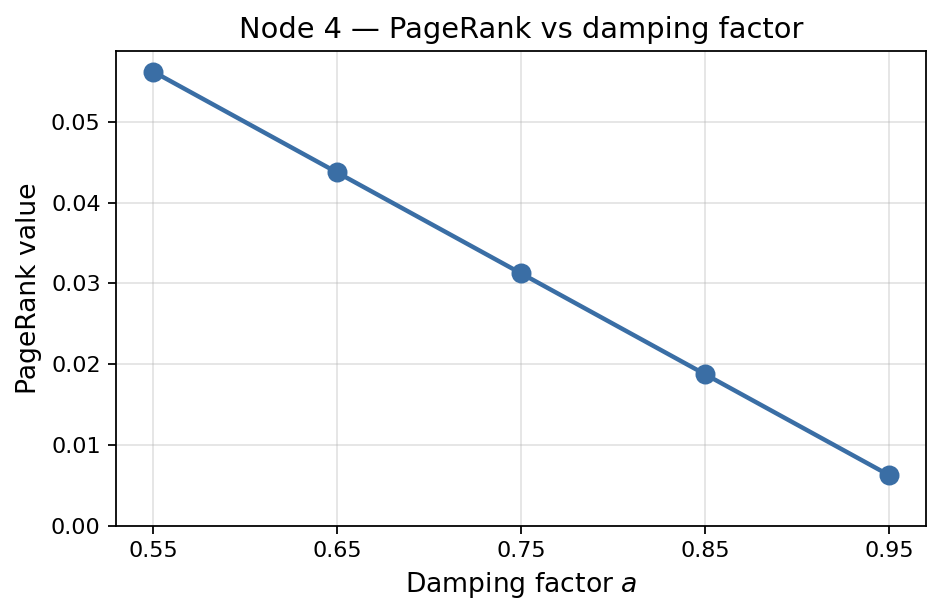
\includegraphics[width=\textwidth]{p1b_node4.png}
    \caption{Node 4}
    \label{fig:p1b_n4}
  \end{subfigure}
  \hfill
  \begin{subfigure}[b]{0.48\textwidth}
    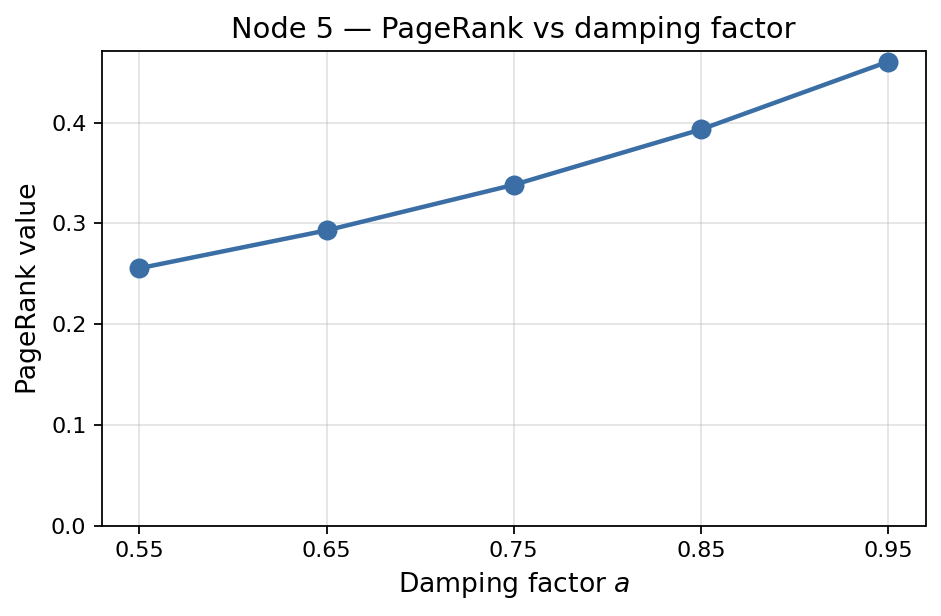
\includegraphics[width=\textwidth]{p1b_node5.png}
    \caption{Node 5}
    \label{fig:p1b_n5}
  \end{subfigure}
  \begin{subfigure}[b]{0.48\textwidth}
    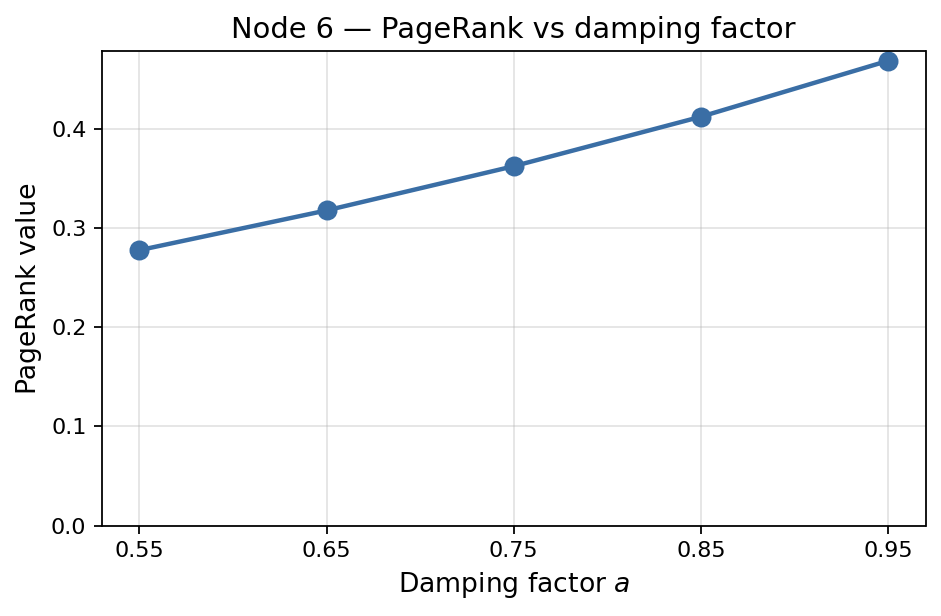
\includegraphics[width=\textwidth]{p1b_node6.png}
    \caption{Node 6}
    \label{fig:p1b_n6}
  \end{subfigure}
  \hfill
  \begin{subfigure}[b]{0.48\textwidth}
    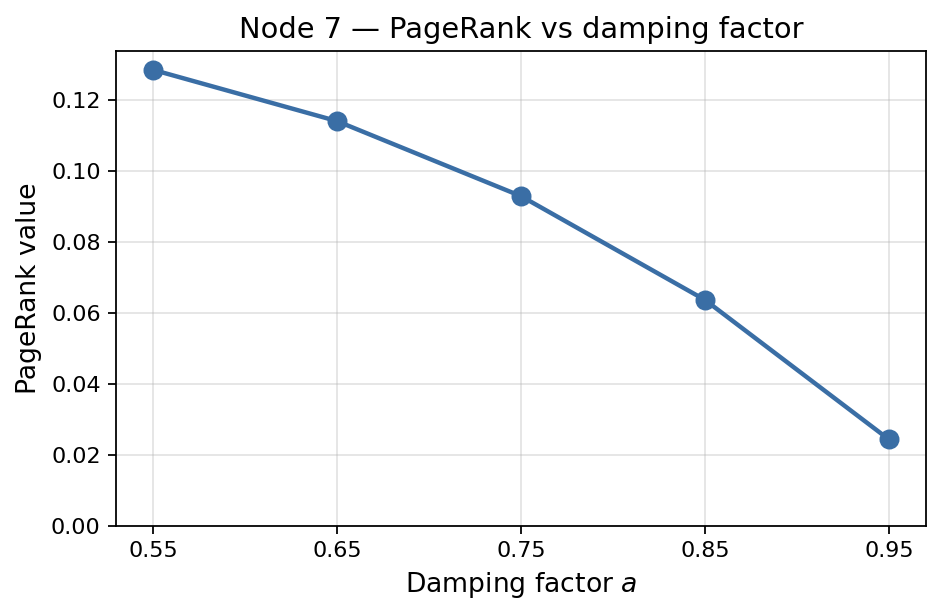
\includegraphics[width=\textwidth]{p1b_node7.png}
    \caption{Node 7}
    \label{fig:p1b_n7}
  \end{subfigure}
  \caption{Part 1B — PageRank vs damping factor, nodes 4--7.}
  \label{fig:p1b_part2}
\end{figure}

\begin{figure}[H]
  \centering
  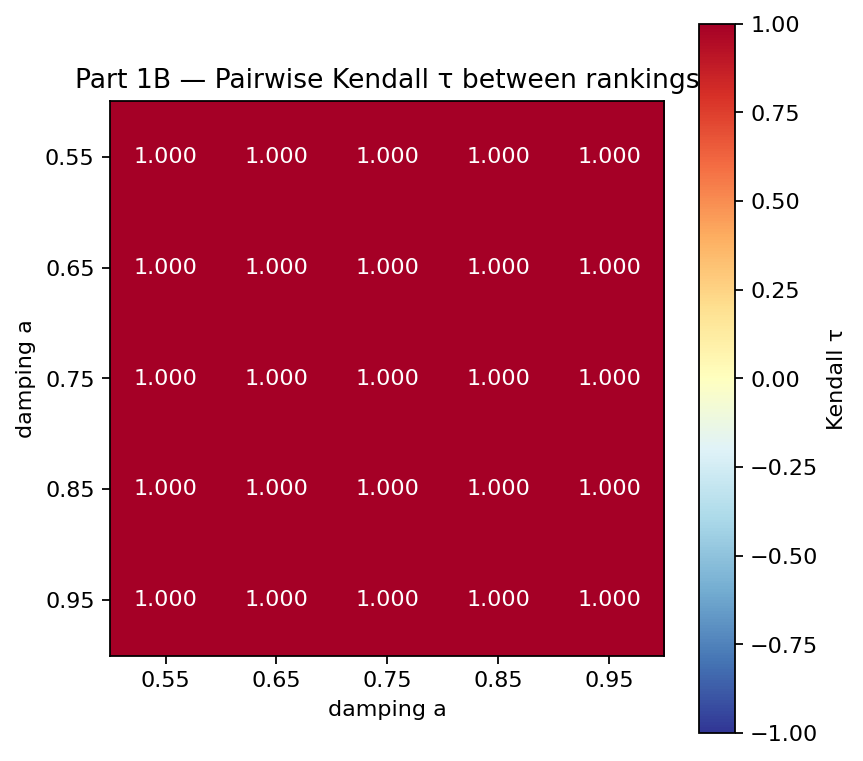
\includegraphics[width=0.55\textwidth]{p1b_kendall_heatmap.png}
  \caption{Pairwise Kendall $\tau$ between the five rankings produced at
           different damping values. All entries are $1.00$.}
  \label{fig:p1b_tau}
\end{figure}

\subsubsection*{Discussion}

From Figures~\ref{fig:p1b_part1}--\ref{fig:p1b_part2}, the absolute PageRank values change
substantially as $a$ increases: nodes~5 and~6---which together form a sink
strongly absorbing random-walk probability (they exchange edges between each
other and receive edges from most other nodes)---see their scores rise sharply
toward $a=0.95$, while all other nodes, whose mass leaks toward 5 and 6,
approach zero. This behaviour is characteristic of nearly-dangling sink
clusters: at high damping the walk spends nearly all its time in the strongly
connected component $\{5,6\}$.

However, the \emph{ranking order} is perfectly stable: every pairwise
Kendall $\tau = 1.00$ (Figure~\ref{fig:p1b_tau}). This means no two nodes
swap positions for any value of $a$ in $[0.55, 0.95]$. The relative
importance hierarchy is determined entirely by graph topology and is
invariant to the damping parameter over this range.

% ─────────────────────────────────────────────────────────────────────
\subsection{Part 1C — HITS on the third graph}

\subsubsection*{Setup}

We applied the HITS algorithm~\cite{kleinberg1999} to the 8-node directed
graph shown in Figure~\ref{fig:p1c_graph}, whose nodes are labelled
$\{2,3,5,7,8,9,10,11\}$.
Authority scores are the principal eigenvector of $A^\top A$;
hub scores are the principal eigenvector of $A A^\top$.
Both matrices are real symmetric positive semi-definite, so we used
\texttt{numpy.linalg.eigh} and took the eigenvector corresponding to the
largest eigenvalue. Results were cross-checked against \texttt{networkx.hits}.

\begin{figure}[H]
  \centering
  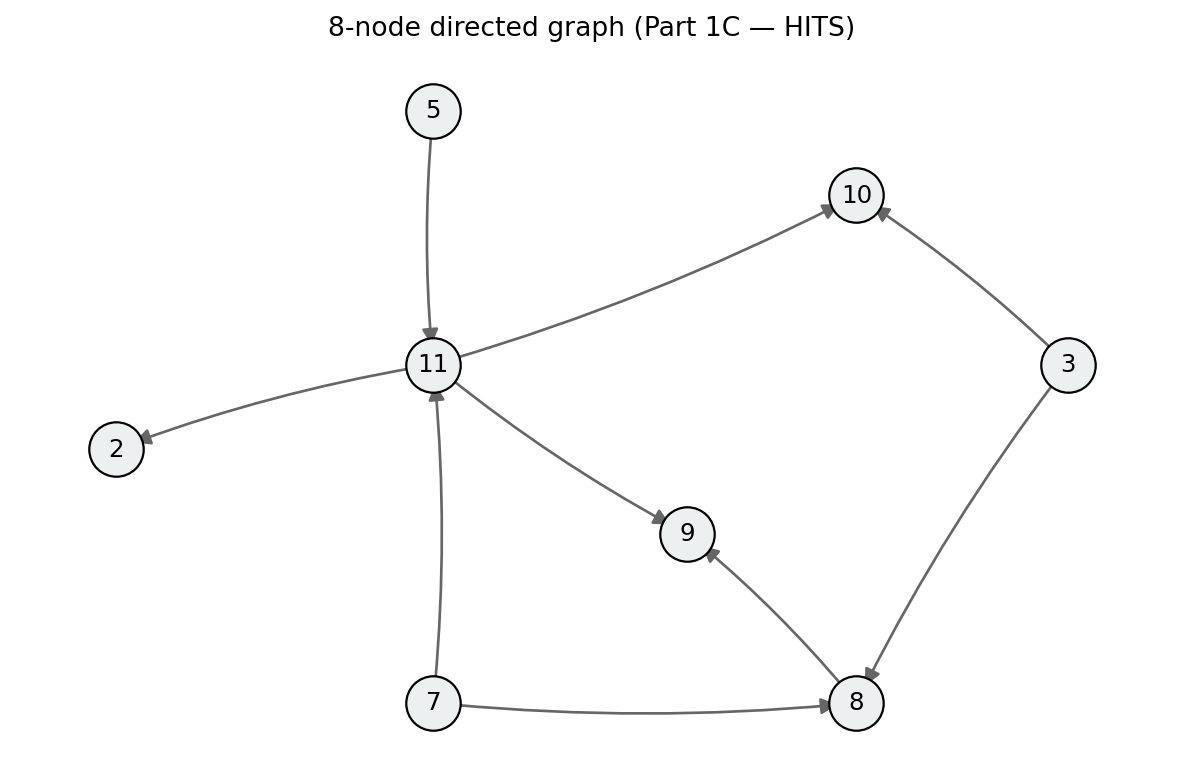
\includegraphics[width=0.60\textwidth]{p1c_graph.png}
  \caption{The directed graph used in Part~1C (HITS).}
  \label{fig:p1c_graph}
\end{figure}

\subsubsection*{Results}

\begin{figure}[H]
  \centering
  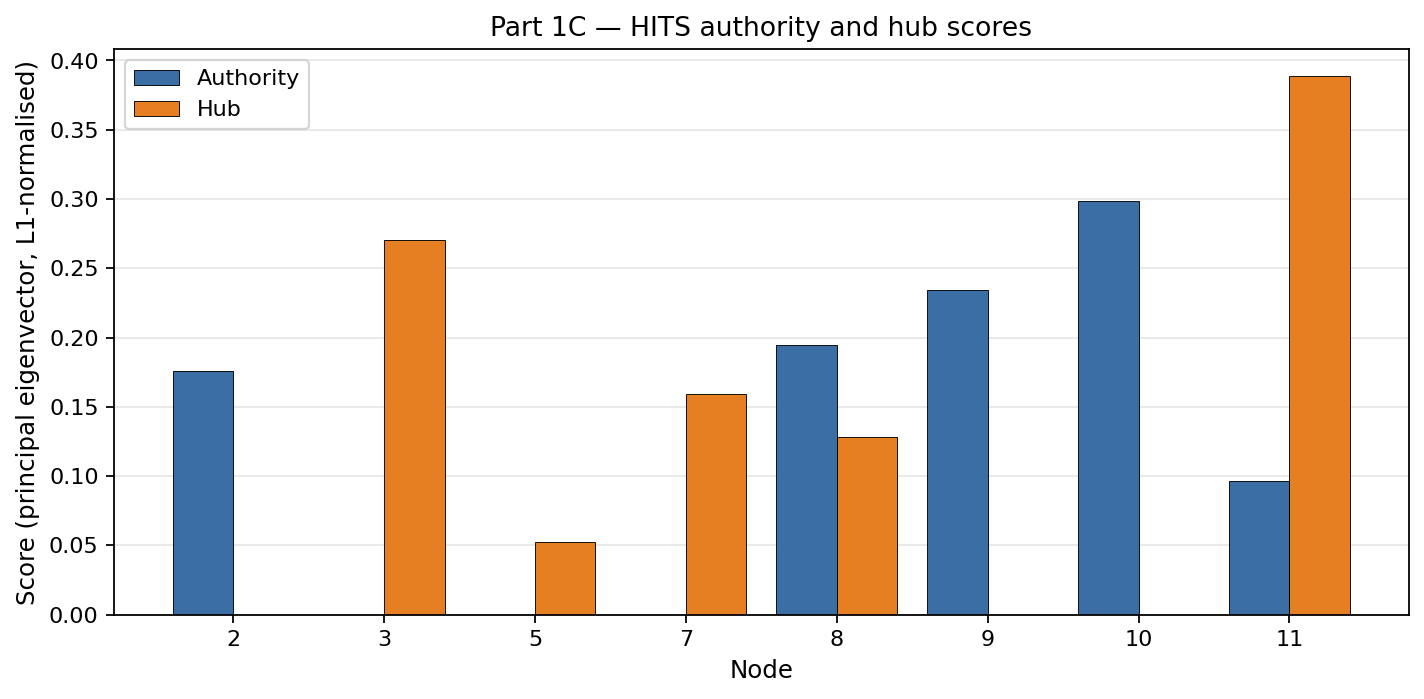
\includegraphics[width=0.92\textwidth]{p1c_hits_scores.png}
  \caption{HITS authority and hub scores for each node (L1-normalised
           principal eigenvectors of $A^\top A$ and $A A^\top$ respectively).}
  \label{fig:p1c_hits}
\end{figure}

\begin{table}[H]
  \centering
  \caption{HITS scores (L1-normalised principal eigenvectors).}
  \label{tab:p1c}
  \begin{tabular}{ccc}
    \toprule
    \textbf{Node} & \textbf{Authority} & \textbf{Hub} \\
    \midrule
    2  & 0.1761 & 0.0000 \\
    3  & 0.0000 & 0.2706 \\
    5  & 0.0000 & 0.0527 \\
    7  & 0.0000 & 0.1595 \\
    8  & 0.1948 & 0.1284 \\
    9  & 0.2343 & 0.0000 \\
    10 & 0.2987 & 0.0000 \\
    11 & 0.0961 & 0.3887 \\
    \bottomrule
  \end{tabular}
\end{table}

\subsubsection*{Discussion}

Authority and hub scores capture complementary structural roles.
\textbf{Node~10} is the top authority (score $0.299$): it receives edges from
node~11 and node~3, both of which are strong hubs, and these hubs point to it
specifically.
\textbf{Node~11} is the top hub (score $0.389$): it has the highest out-degree
in the graph (edges to nodes 2, 9, and 10) and is pointed to by both node~5
and node~7.

Nodes with zero hub score (2, 9, 10) have no outgoing edges and are pure
sinks; nodes with zero authority score (3, 5, 7) have no incoming edges from
other hubs and are pure sources.
Node~8 is the only node that plays both roles meaningfully (authority $0.195$,
hub $0.128$): it both receives an edge from node~3 (a hub) and emits an edge
to node~9 (boosting its hub score).

% ─────────────────────────────────────────────────────────────────────
\subsection{Part 1D — Eigenvalues of the Google matrix}

\subsubsection*{Setup}

We computed the eigenvalues of the Google matrix
\[
  G = a M + \frac{1-a}{n} \mathbf{1}\mathbf{1}^\top
\]
for the 14-node graph at $a = 0.85$, where $M$ is the row-stochastic
transition matrix. We then added the five cross-cluster edges
$(5{-}11),\ (4{-}11),\ (7{-}13),\ (8{-}12),\ (9{-}13)$
and recomputed the eigenvalues of the modified graph.

\subsubsection*{Results}

\begin{figure}[H]
  \centering
  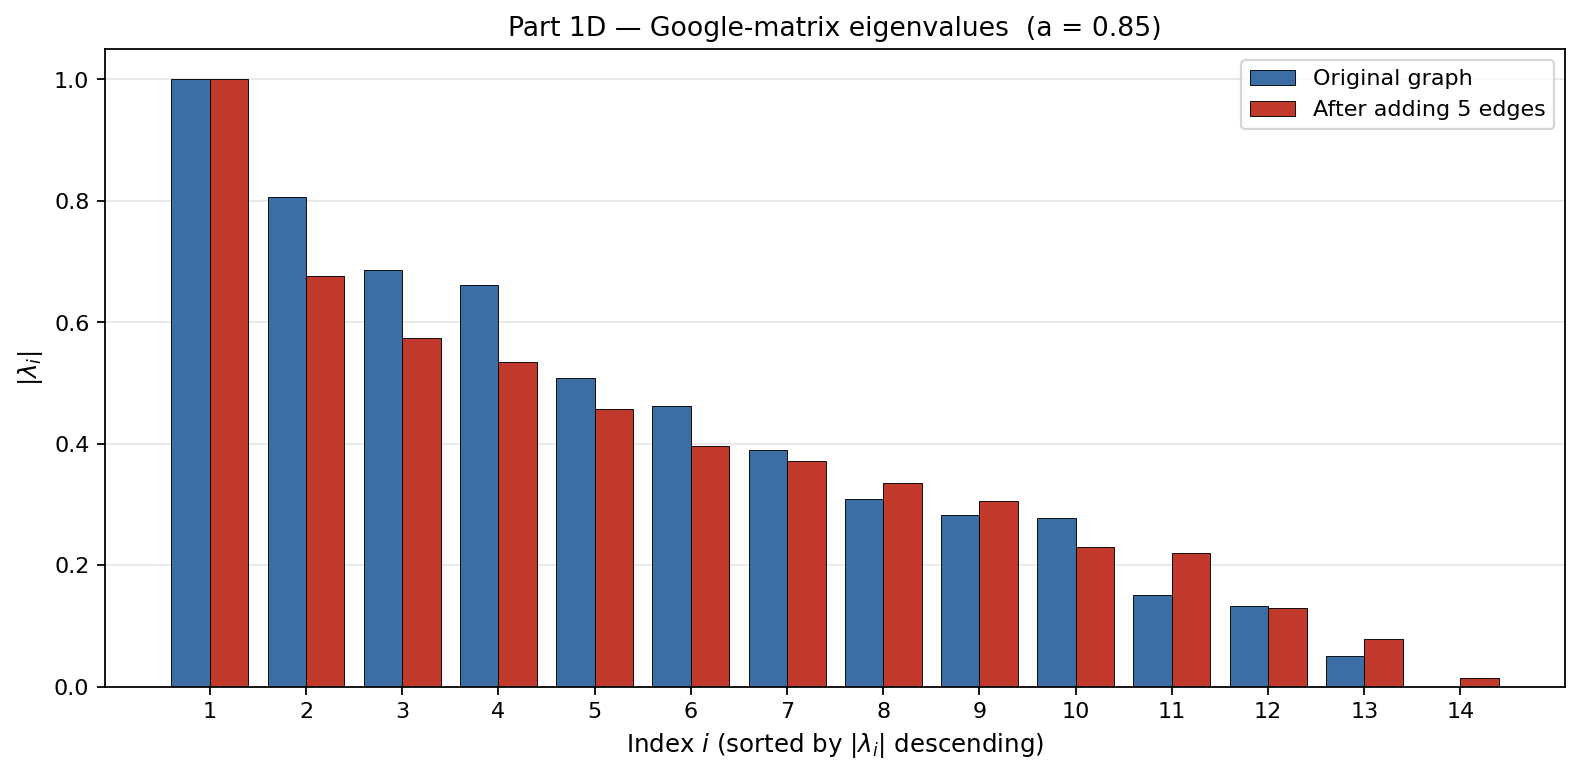
\includegraphics[width=0.95\textwidth]{p1d_eigenvalues.png}
  \caption{Magnitudes of the Google-matrix eigenvalues before and after
           adding five cross-cluster edges ($a=0.85$).}
  \label{fig:p1d_eig}
\end{figure}

\begin{table}[H]
  \centering
  \caption{Key spectral quantities before and after edge addition.}
  \label{tab:p1d}
  \begin{tabular}{lcc}
    \toprule
    \textbf{Quantity} & \textbf{Original} & \textbf{Modified} \\
    \midrule
    $|\lambda_1|$          & 1.0000 & 1.0000 \\
    $|\lambda_2|$          & 0.8071 & 0.6769 \\
    Spectral gap $(1-|\lambda_2|)$ & 0.1929 & 0.3231 \\
    Number of edges        & 22     & 27     \\
    \bottomrule
  \end{tabular}
\end{table}

\subsubsection*{Discussion}

The dominant eigenvalue $\lambda_1 = 1$ is invariant in both cases: any
row-stochastic matrix has spectral radius exactly~1.

The key quantity is $|\lambda_2|$, which controls the convergence rate of the
power iteration used to compute PageRank: the error after $t$ iterations
decays as $\mathcal{O}(|\lambda_2|^t)$, so a smaller $|\lambda_2|$ means
faster convergence.

\textbf{Original graph.} The three weakly-coupled clusters connected by
single-bridge edges produce an $|\lambda_2| = 0.807$, close to the theoretical
ceiling of $a = 0.85$. The Markov chain mixes slowly because a random walk
can be ``trapped'' in one cluster for many steps.

\textbf{Modified graph.} Adding five cross-cluster edges reduces
$|\lambda_2|$ to $0.677$, and the spectral gap nearly doubles from $0.193$
to $0.323$.  The new edges directly connect the previously
isolated clusters, creating shorter paths between all pairs of nodes and
making the stationary distribution easier to reach from any starting point.
The remaining eigenvalues $|\lambda_3|, \dots, |\lambda_{14}|$ also
compress uniformly downward (visible in Figure~\ref{fig:p1d_eig}), reflecting
the more uniform mixing geometry of the modified graph.

% ═════════════════════════════════════════════════════════════════════
\section{Part 2 — Zipf's Law on \textit{Pride and Prejudice} (1 point)}
% ═════════════════════════════════════════════════════════════════════

\subsection{Setup}

We tested Zipf's law~\cite{zipf1949} on Jane Austen's
\textit{Pride and Prejudice} (Project Gutenberg eBook \#1342,
Plain Text UTF-8~\cite{gutenberg1342}).
The text was stripped of Project Gutenberg boilerplate and tokenised
with the regex \texttt{[a-z]+(?:'[a-z]+)?}, which preserves contractions
as single tokens (e.g.\ \textit{don't}) and lower-cases all words.
\textbf{No stemming} was applied.

Zipf's law states that the collection frequency of the $i$-th most
frequent term satisfies
\[
  \mathrm{cf}_i \approx \frac{c}{i},
\]
i.e.\ in log-log space the frequency--rank curve is a straight line
with slope $-1$.

The constant $c$ was estimated by three methods:
\begin{enumerate}
  \item $c_a = \mathrm{cf}_1$ (the most-frequent term's count).
  \item $c_b = \text{median}(\mathrm{cf}_i \cdot i)$ across all ranks.
  \item $c_c$: least-squares fit of $\log \mathrm{cf}_i = \log c - b \log i$
        over the top 1\,000 ranks.
\end{enumerate}
Estimator (c) is the primary result; the fit also yields the empirical
exponent $b$ (Zipf predicts $b = 1$).

\subsection{Results}

\begin{figure}[H]
  \centering
  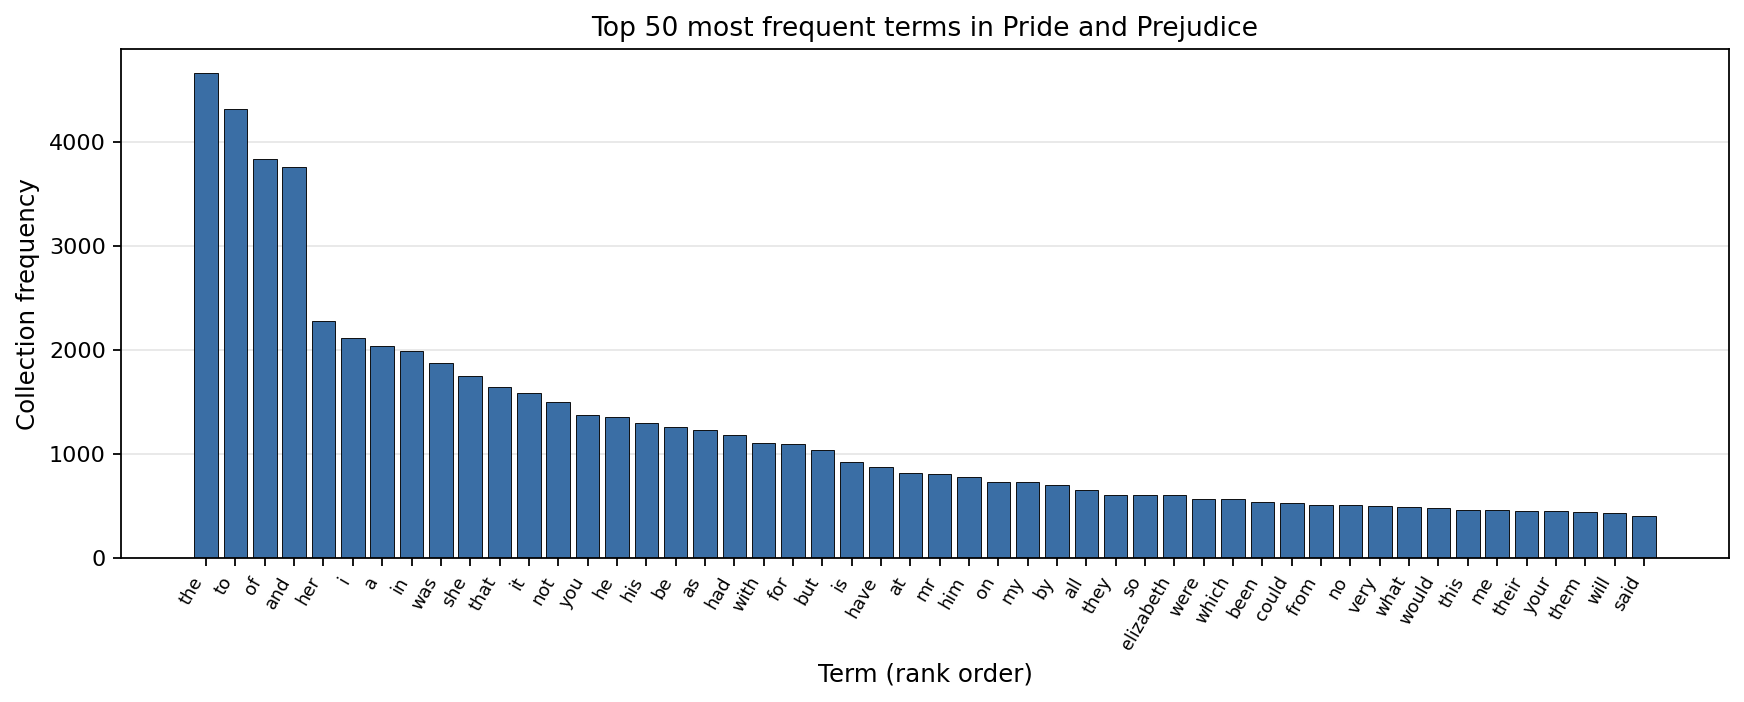
\includegraphics[width=0.95\textwidth]{zipf_top50_bar.png}
  \caption{Collection frequencies of the 50 most frequent terms in
           \textit{Pride and Prejudice}.}
  \label{fig:zipf_bar}
\end{figure}

\begin{figure}[H]
  \centering
  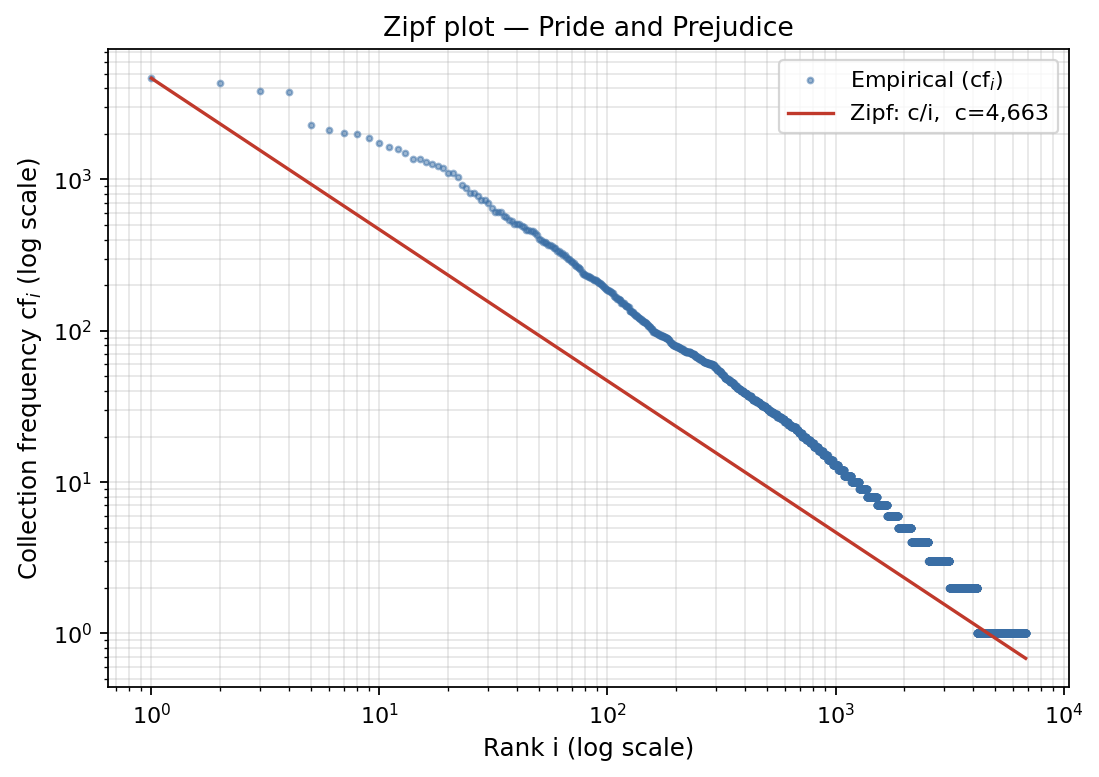
\includegraphics[width=0.80\textwidth]{zipf_loglog.png}
  \caption{Log-log Zipf plot. Blue dots: empirical frequencies.
           Red line: fitted model $c/i$, $c = 24\,874$.}
  \label{fig:zipf_loglog}
\end{figure}

\begin{table}[H]
  \centering
  \caption{Estimates of the Zipf constant $c$ for
           \textit{Pride and Prejudice}.}
  \label{tab:zipf}
  \begin{tabular}{lc}
    \toprule
    \textbf{Estimator} & \textbf{$c$} \\
    \midrule
    (a) $\mathrm{cf}_1$ (``the'')          & 4\,663 \\
    (b) $\text{mean}(\mathrm{cf}_i \cdot i)$  & 8\,734 \\
    (b) $\text{median}(\mathrm{cf}_i \cdot i)$& 7\,788 \\
    (c) log-log fit (top 1\,000 ranks)     & \textbf{24\,874} \\
    \midrule
    Empirical exponent $b$                 & \textbf{1.080} \\
    \bottomrule
  \end{tabular}
\end{table}

\subsection{Discussion}

Zipf's law is clearly confirmed for this corpus.
The log-log plot (Figure~\ref{fig:zipf_loglog}) exhibits a near-straight
decay over roughly two decades of rank, and the fitted exponent
$b = 1.080$ is within $8\%$ of Zipf's theoretical prediction of $1.0$.

The spread across the three estimators (4\,663 to 24\,874) is expected
and does not indicate inconsistency.
The $c_a$ estimator uses a single data point (``the'', 4\,663 occurrences),
which lies \emph{below} the fitted line---a well-documented phenomenon
at the extreme head of the distribution (the Mandelbrot correction).
The log-log fit intercepts at rank~1 but the actual slope $-1.08$
is slightly steeper than $-1$, extrapolating to a higher value of~$c$
at rank~1 than is actually observed.

The top-50 bar chart (Figure~\ref{fig:zipf_bar}) shows the characteristic
sharp falloff after the first handful of function words
(\textit{the}, \textit{to}, \textit{of}, \textit{and}, \textit{her}).
The appearance of ``elizabeth'' at rank~29 and ``mr'' at rank~23 is
domain-specific: these are character references, not generic function
words, and their relatively high frequency reflects the novel's focus on
the Bennet family and Mr.\ Darcy.

Deviations from the model are concentrated in two regions:
(i) the \emph{head} (ranks 1--15), where function words are slightly
below the fit due to the Mandelbrot effect, and
(ii) the \emph{tail}, where hapax legomena (words appearing exactly once)
form a flat staircase that falls well below the extrapolated line.

% ═════════════════════════════════════════════════════════════════════
\section{Part 3 — Bayesian Personalised Ranking (5 points)}
% ═════════════════════════════════════════════════════════════════════

\subsection{Setup}

We implemented Bayesian Personalised Ranking (BPR)~\cite{rendle2009bpr}
for top-$k$ recommendation on two datasets:

\begin{itemize}
  \item \textbf{Last.FM} (HetRec 2011~\cite{cantador2011}):
        1\,892 users, 17\,632 artists, 92\,834 user--artist interactions.
        Any listening event is treated as a positive signal.
  \item \textbf{MovieLens 1M}~\cite{harper2015movielens}:
        6\,040 users, 3\,706 movies, 1\,000\,209 ratings.
        Any rating (regardless of value) is treated as a positive interaction.
\end{itemize}

\textbf{Split:} per user, 80\% of interactions are kept for training and
20\% are held out for testing. Users with fewer than 2 interactions remain
entirely in the training set.

\textbf{Evaluation protocol:} each experiment is repeated \textbf{10 times}
with different random seeds for the train/test split.
Results report \textbf{mean $\pm$ std} over these 10 runs.

\textbf{Implementation:} BPR matrix factorisation from the
\texttt{implicit} library (v0.7.2, Cython backend), with
\texttt{iterations=100}, \texttt{learning\_rate=0.01},
\texttt{regularization=0.01}.

\textbf{Metrics:}
\[
  \text{Precision@}k = \frac{|\text{recommended} \cap \text{relevant}|}{k},
  \qquad
  \text{Recall@}k = \frac{|\text{recommended} \cap \text{relevant}|}{|\text{relevant}|}.
\]

% ─────────────────────────────────────────────────────────────────────
\subsection{Part 3A — Effect of latent factors (top-10 recommendation)}

We fixed $k = 10$ and varied the number of latent factors
$f \in \{10, 20, \ldots, 100\}$.

\begin{figure}[H]
  \centering
  \begin{subfigure}[b]{0.48\textwidth}
    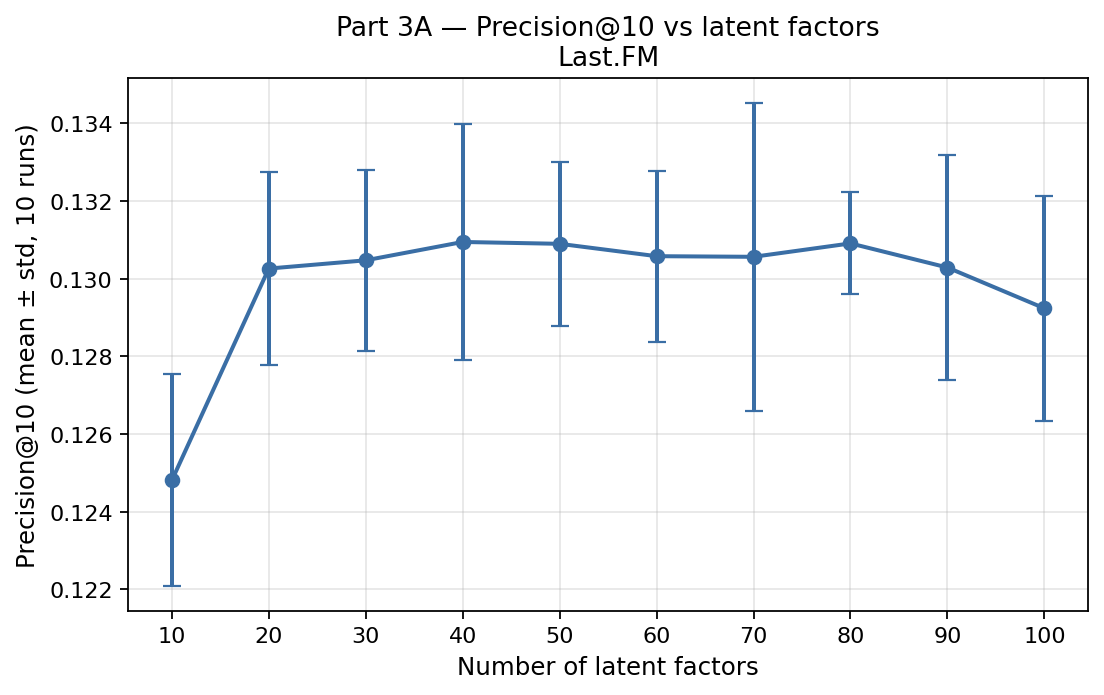
\includegraphics[width=\textwidth]{p3a_precision_lastfm.png}
    \caption{Precision@10 — Last.FM}
    \label{fig:p3a_prec_lfm}
  \end{subfigure}
  \hfill
  \begin{subfigure}[b]{0.48\textwidth}
    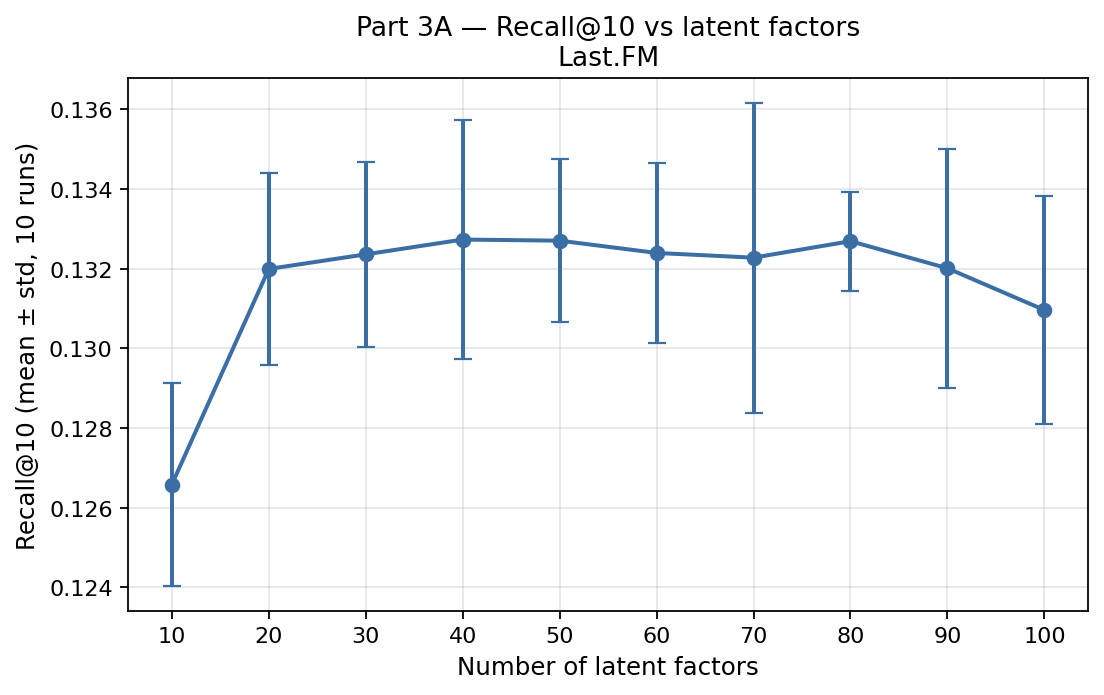
\includegraphics[width=\textwidth]{p3a_recall_lastfm.png}
    \caption{Recall@10 — Last.FM}
    \label{fig:p3a_rec_lfm}
  \end{subfigure}
  \begin{subfigure}[b]{0.48\textwidth}
    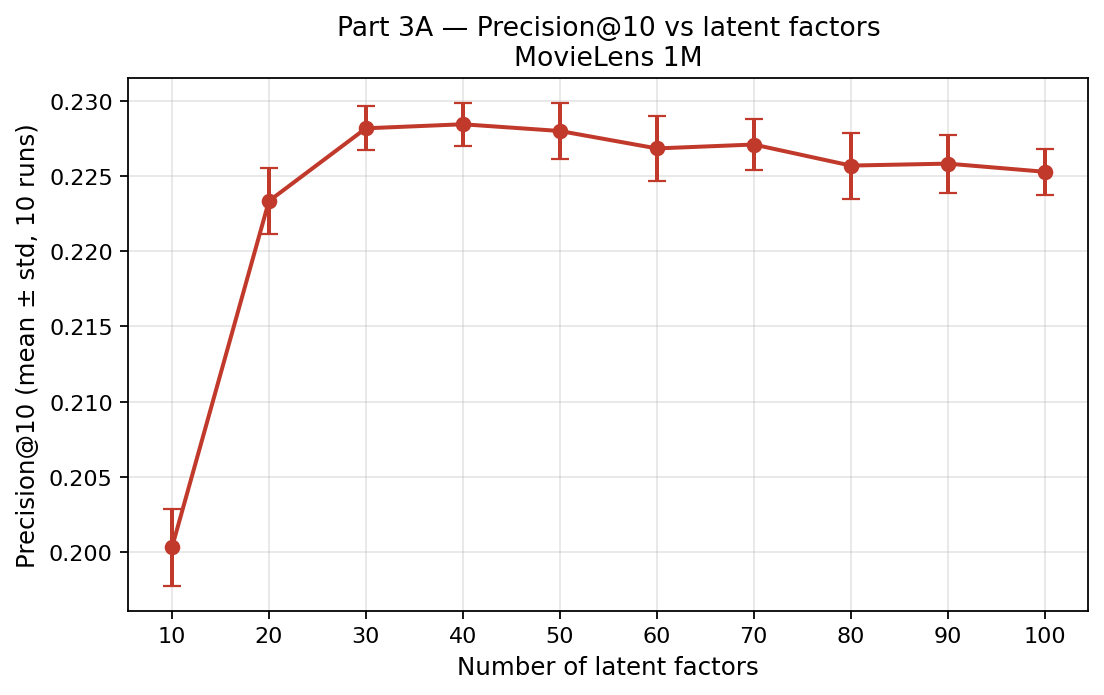
\includegraphics[width=\textwidth]{p3a_precision_ml1m.png}
    \caption{Precision@10 — MovieLens 1M}
    \label{fig:p3a_prec_ml}
  \end{subfigure}
  \hfill
  \begin{subfigure}[b]{0.48\textwidth}
    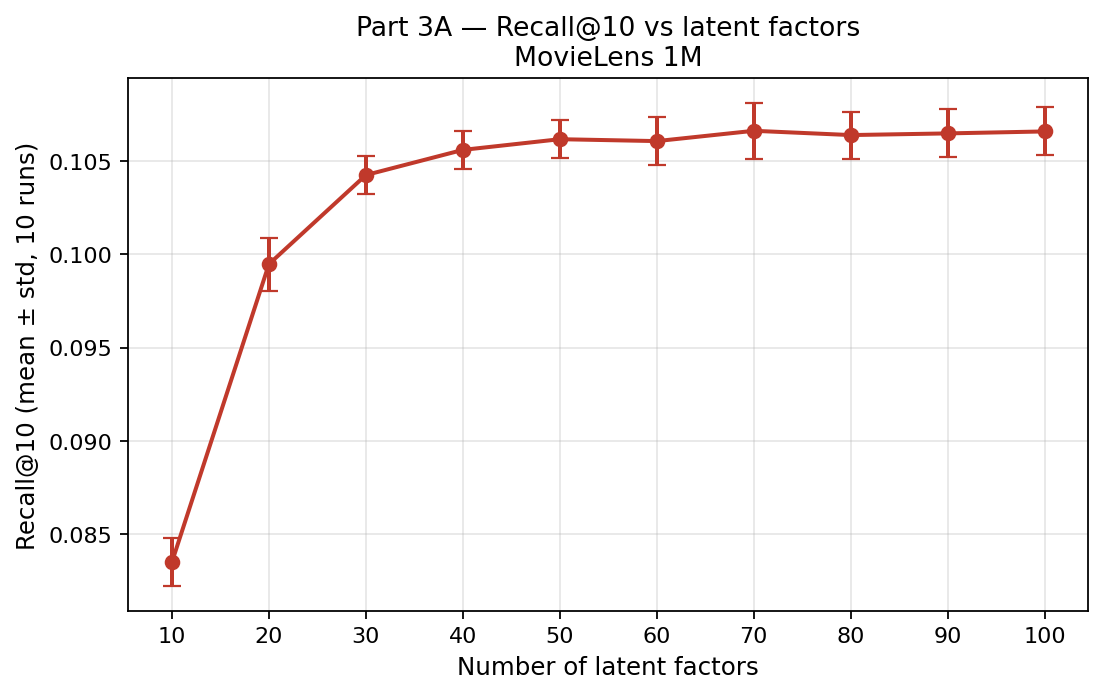
\includegraphics[width=\textwidth]{p3a_recall_ml1m.png}
    \caption{Recall@10 — MovieLens 1M}
    \label{fig:p3a_rec_ml}
  \end{subfigure}
  \caption{Part 3A: Precision@10 and Recall@10 as a function of the number of
           latent factors ($k=10$, 10 runs each, error bars = $\pm$1 std).}
  \label{fig:p3a}
\end{figure}

\subsubsection*{Discussion}

Both datasets show a fast initial gain from $f=10$ to $f=30$, after which
performance plateaus and then very slightly declines toward $f=100$.
The saturation indicates that the preference space of these datasets is
well-captured by $\approx30$ latent dimensions; adding more factors does
not improve generalisation and may introduce mild overfitting to training
interactions.

MovieLens 1M consistently outperforms Last.FM on Precision@10
(peak $\approx 0.228$ vs $\approx 0.131$) because it is a denser dataset
with more interactions per user, giving the model more signal to learn from.
On Recall@10 the gap is inverted: Last.FM achieves higher recall
($\approx 0.133$ vs $\approx 0.106$) because its item catalogue is larger
relative to the number of users, so the 20\% held-out set contains more
items and each correctly recommended item yields a larger recall gain.

The standard deviations across 10 runs are consistently small
(below $0.004$), confirming that the results are stable and not
sensitive to the particular train/test split.

% ─────────────────────────────────────────────────────────────────────
\subsection{Part 3B — Effect of $k$ (fixed factors = 50)}

We fixed the number of latent factors to 50 and varied
$k \in \{2, 4, 6, \ldots, 20\}$.

\begin{figure}[H]
  \centering
  \begin{subfigure}[b]{0.48\textwidth}
    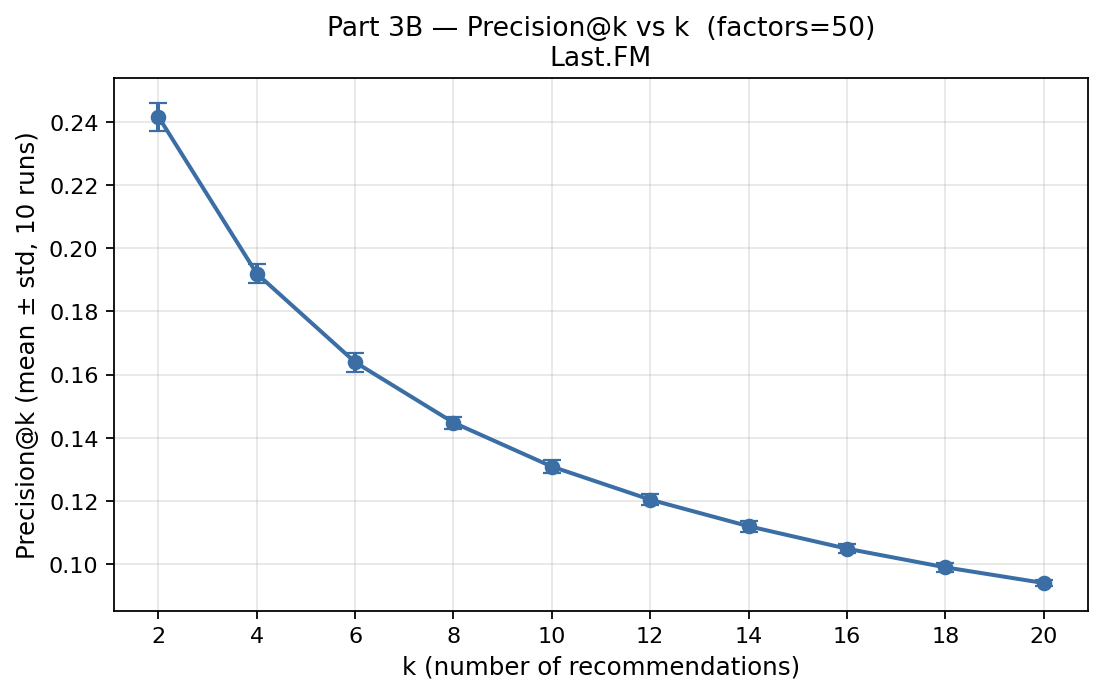
\includegraphics[width=\textwidth]{p3b_precision_lastfm.png}
    \caption{Precision@k — Last.FM}
    \label{fig:p3b_prec_lfm}
  \end{subfigure}
  \hfill
  \begin{subfigure}[b]{0.48\textwidth}
    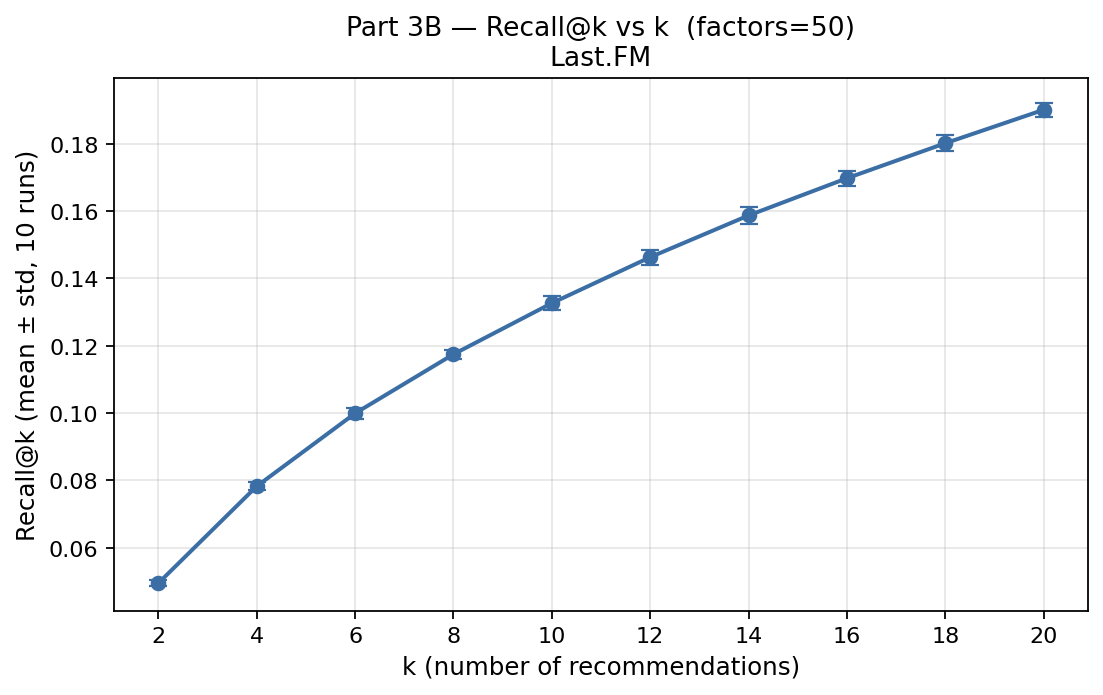
\includegraphics[width=\textwidth]{p3b_recall_lastfm.png}
    \caption{Recall@k — Last.FM}
    \label{fig:p3b_rec_lfm}
  \end{subfigure}
  \begin{subfigure}[b]{0.48\textwidth}
    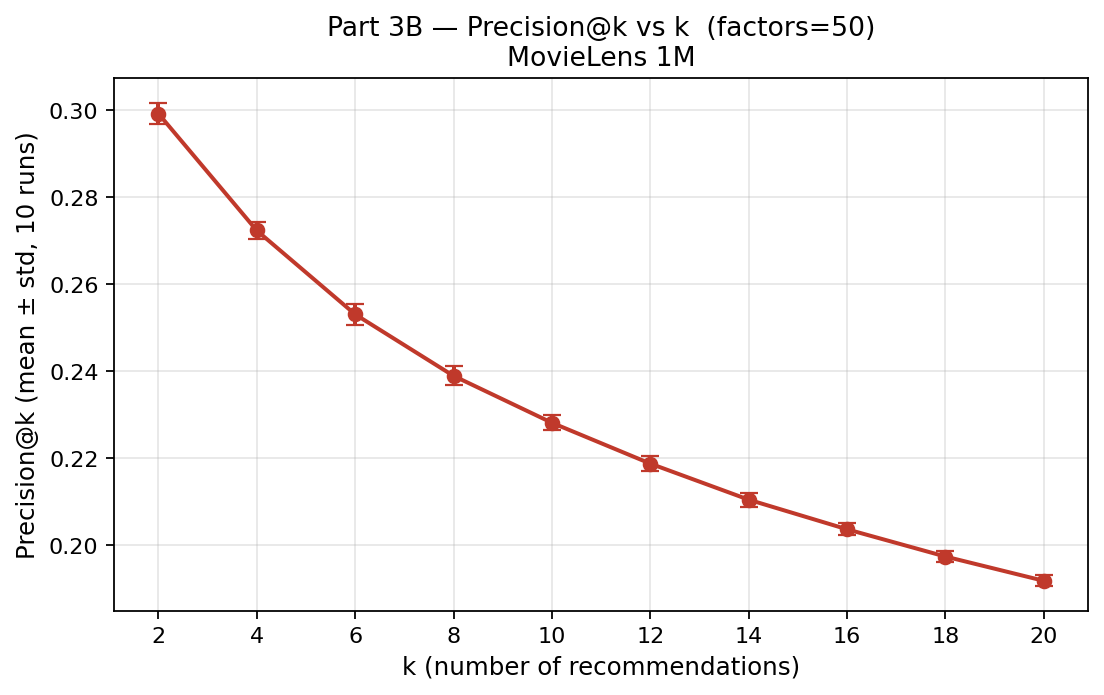
\includegraphics[width=\textwidth]{p3b_precision_ml1m.png}
    \caption{Precision@k — MovieLens 1M}
    \label{fig:p3b_prec_ml}
  \end{subfigure}
  \hfill
  \begin{subfigure}[b]{0.48\textwidth}
    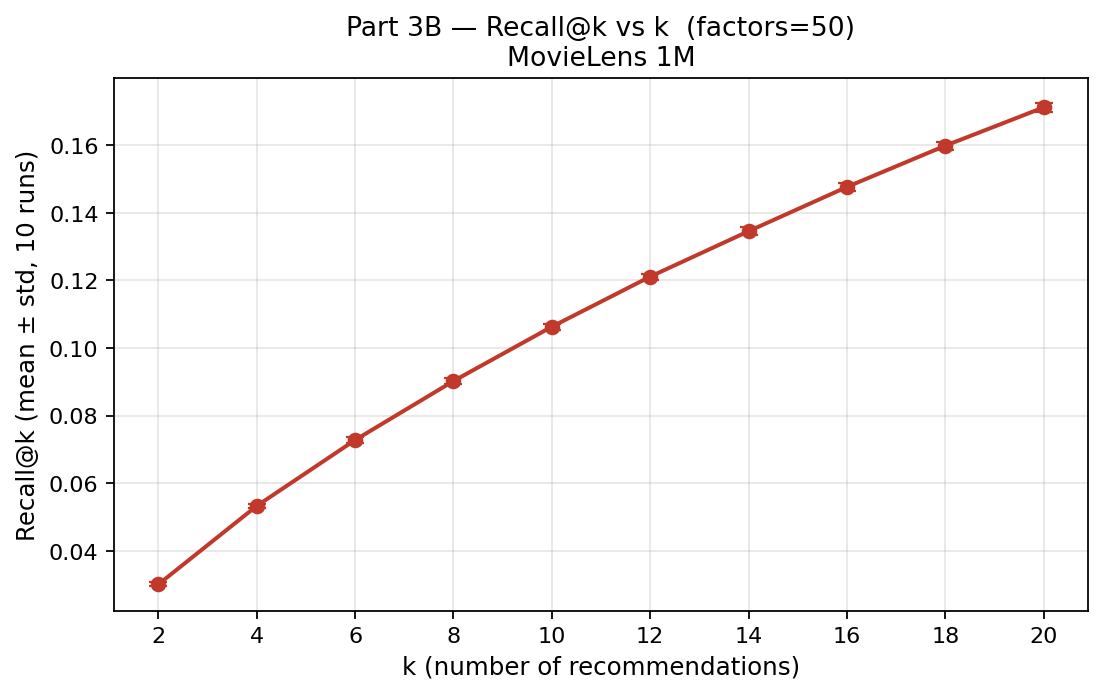
\includegraphics[width=\textwidth]{p3b_recall_ml1m.png}
    \caption{Recall@k — MovieLens 1M}
    \label{fig:p3b_rec_ml}
  \end{subfigure}
  \caption{Part 3B: Precision@k and Recall@k as a function of $k$
           (factors=50, 10 runs each, error bars = $\pm$1 std).}
  \label{fig:p3b}
\end{figure}

\subsubsection*{Discussion}

The results exhibit the classic precision--recall trade-off:

\textbf{Precision@k} decreases monotonically as $k$ grows.
At $k=2$, the model recommends only its two most confident items, so
the hit rate is high (Last.FM: $0.242$; MovieLens~1M: $0.299$).
As $k$ increases, the list is padded with less-confident recommendations,
diluting precision.

\textbf{Recall@k} increases monotonically with $k$.
A longer list captures more of the held-out items, improving recall.
At $k=20$, Last.FM recall reaches $0.190$ and MovieLens~1M reaches $0.171$.

MovieLens~1M maintains higher precision than Last.FM across all $k$
values, consistent with the denser interaction matrix giving the model
better estimates of user preferences.
Last.FM achieves higher recall at larger $k$, consistent with the
explanation given in Part~3A (larger item space, fewer interactions per
user, more diverse held-out sets).

The error bars remain very tight throughout, confirming the robustness
of the 10-repetition protocol.

% ═════════════════════════════════════════════════════════════════════
\section{Conclusions}
% ═════════════════════════════════════════════════════════════════════

This report covered three topics in information retrieval.

In \textbf{Part~1} we studied link-analysis algorithms on small graphs.
Personalised PageRank concentrates importance near the teleport target,
overriding the topological hierarchy. The PageRank ranking on the directed
graph is perfectly stable across all tested damping factors ($\tau=1$ for
all pairs), while the absolute scores shift substantially. HITS cleanly
separates hub and authority roles, identifying nodes that either point to
many good sources or are pointed to by many good hubs. Finally, adding
cross-cluster edges to a weakly-connected graph nearly doubles the spectral
gap of the Google matrix, accelerating the convergence of power iteration.

In \textbf{Part~2} we confirmed Zipf's law on \textit{Pride and Prejudice}.
The empirical exponent $b = 1.080$ is within $8\%$ of the theoretical
prediction of $1.0$, and the log-log plot is approximately straight over
two decades of rank. Deviations at the head and tail are consistent with
the known Mandelbrot correction and the discrete nature of hapax legomena.

In \textbf{Part~3} we applied BPR to implicit-feedback recommendation on
two real datasets. Performance saturates at roughly 30 latent factors on
both datasets, suggesting that the user-preference space is low-dimensional.
The precision--recall trade-off as $k$ varies is clean and monotone,
confirming that BPR produces well-calibrated rankings.

\textbf{Software.} All experiments were implemented in Python~3.12 using
\texttt{networkx} (graph algorithms), \texttt{numpy}/\texttt{scipy}
(linear algebra), \texttt{matplotlib} (figures), \texttt{pandas}
(tabulation), and \texttt{implicit} (BPR).
All code is available at
\url{https://github.com/mavroul1s/ir-assignment-2026}.

% ═════════════════════════════════════════════════════════════════════
\bibliographystyle{plain}
\bibliography{refs}
% ═════════════════════════════════════════════════════════════════════

\end{document}
